\chapter{Implementazione}

Il software è stato scritto in Prolog, in particolare utilizzando SWI-Prolog ver. 7.2.0. Mentre per la parte grafica è stato utilizzato Java ver. 1.8. Il sistema operativo è Ubuntu Desktop 64-bit 15.10.

\section{Struttura}
Per sviluppare le funzionalità del sistema sono stati realizzati dei moduli in formato \texttt{.pl}, che sono elencati di seguito:
\begin{itemize}
\item \texttt{main}: il punto di accesso del sistema per la riga di comando.
\item \texttt{menu\_utente}: presenta un menu utilizzabile da utenti normali.
\item \texttt{menu\_admin}: presenta un menu utilizzabile da utenti con privilegi.
\item \texttt{circolazione}: il cuore del sistema, si occupa della risoluzione degli incroci.
\item \texttt{precedenze}: gestisce come i veicoli diano o abbiano la precedenza sugli altri.
\item \texttt{deadlock}: gestisce gli stalli.
\item \texttt{destra}: descrive come un veicolo sia a destra di un altro.
\item \texttt{gestore\_kb}: permette l'accesso in lettura e scrittura della \emph{knowledge base}.
\item \texttt{java\_access\_point}: interfaccia di comunicazione con il programma Java, fornito di una GUI.
\item \texttt{adiacenza}: descrive come un braccio sia adiacente ad un altro.
\item \texttt{opposti}: descrive come un veicolo sia opposto ad un altro.
\item \texttt{posizioni}: descrive casi particolari di come sono situati i veicoli.
\item \texttt{prioritari}: definisce vari gradi di priorità e quali tipi di veicoli ne godono.
\item \texttt{segnali}: definisce i segnali stradali presenti nell'incrocio.
\item \texttt{msg}: messaggi di output \emph{user-friendly}.
\item \texttt{utils}: fornisce diversi metodi di utilità.
\end{itemize}

Inoltre la base di conoscenza è salvata nel file \texttt{kb.pl}, che contiene gli incroci già pronti per essere risolti.

\newgeometry{left=1cm, right=1cm}
\begin{figure}
	\makebox[\textwidth]{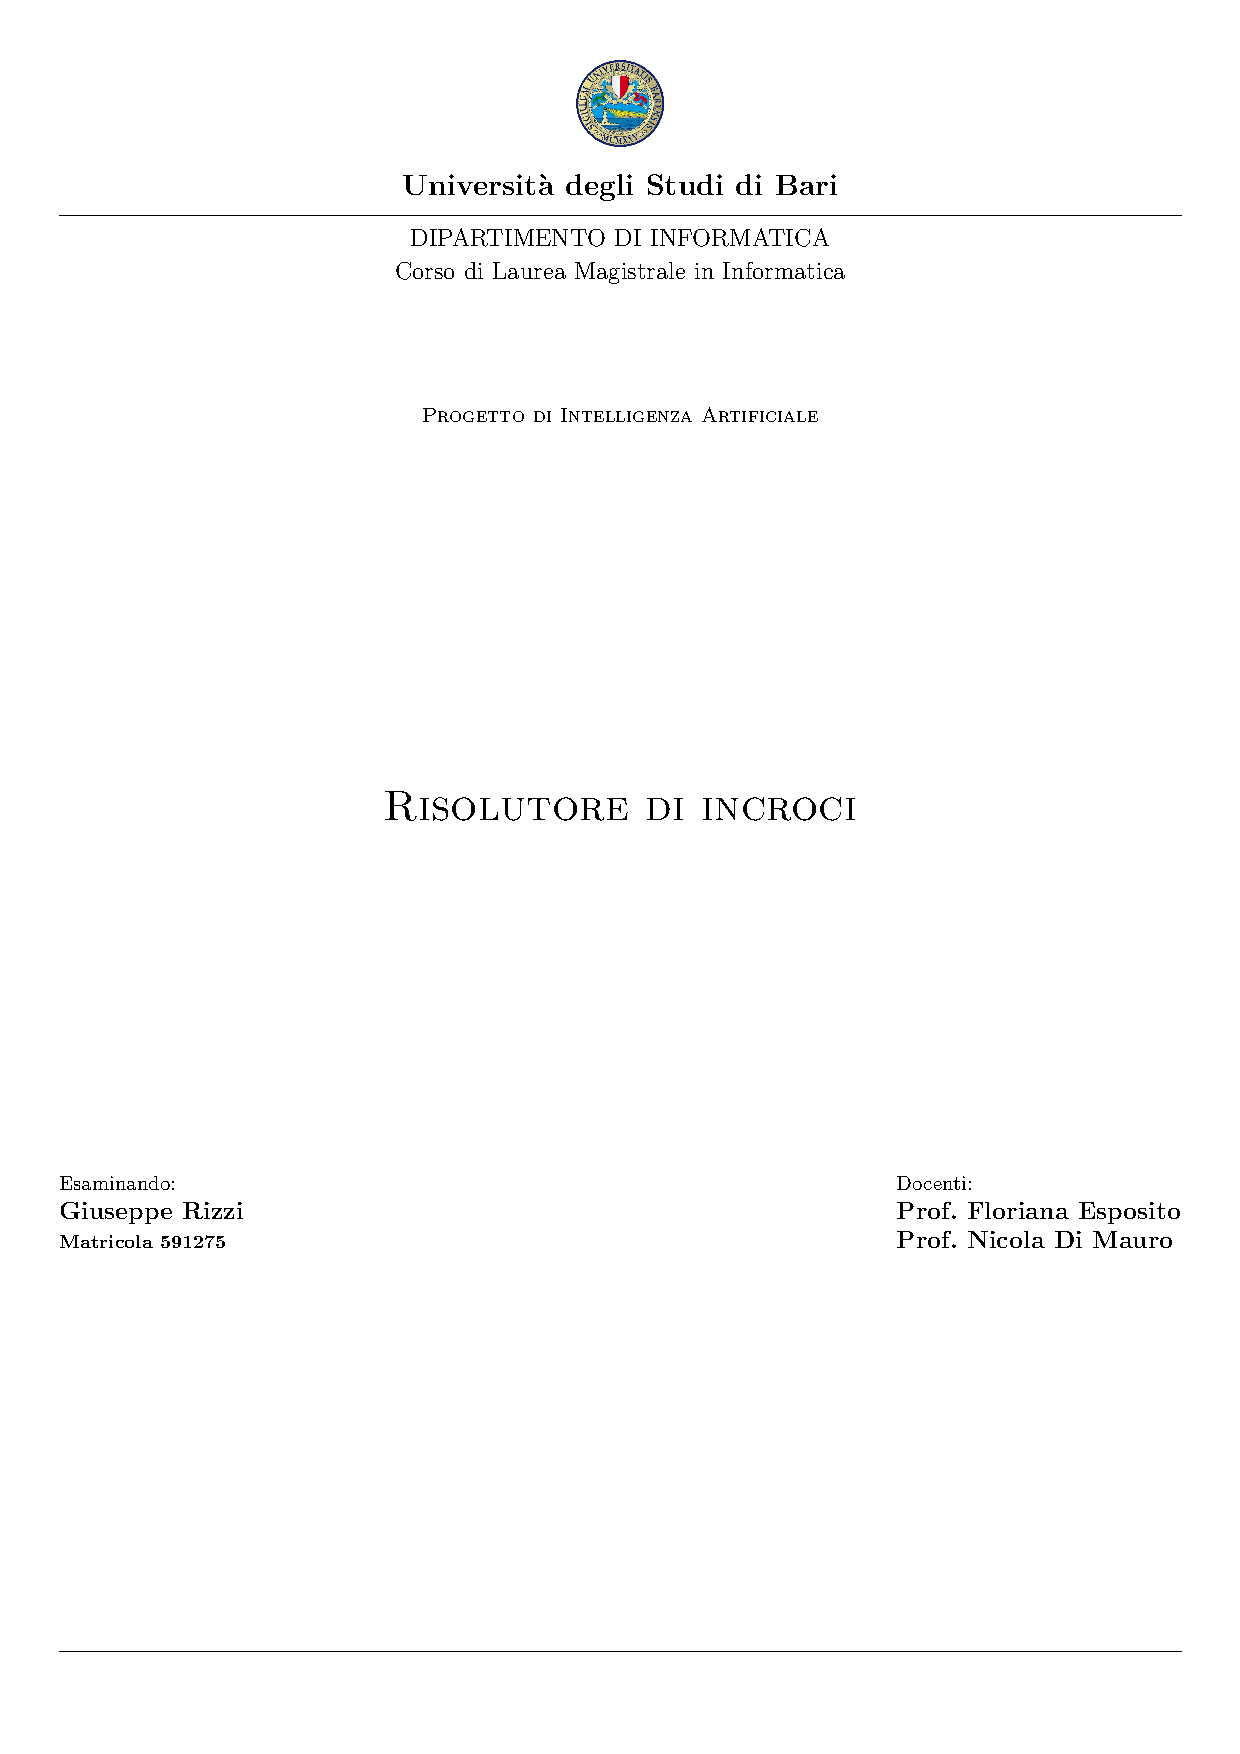
\includegraphics[width=1.2\textwidth]{code/diagrams/main}}
	\caption{\texttt{main.pl}}
\end{figure}

\begin{figure}
	\makebox[\textwidth]{\includegraphics[width=1.2\textwidth]{code/diagrams/menu_utente}}
	\caption{\texttt{menu\_utente.pl}}
\end{figure}

\begin{figure}
	\makebox[\textwidth]{\includegraphics[width=1.2\textwidth]{code/diagrams/menu_admin}}
	\caption{\texttt{menu\_admin.pl}}
\end{figure}
\restoregeometry


\newgeometry{top=1mm, bottom=1mm}
\begin{sidewaysfigure}
	\thisfloatpagestyle{empty}
	\includegraphics[width=\textwidth, height=\textheight, keepaspectratio]{code/diagrams/circolazione}
	\caption{\texttt{circolazione.pl}}
\end{sidewaysfigure}

\begin{sidewaysfigure}
	\thisfloatpagestyle{empty}
	\includegraphics[width=\textwidth, height=\textheight, keepaspectratio]{code/diagrams/precedenze}
	\caption{\texttt{precedenze.pl}}
\end{sidewaysfigure}

\begin{sidewaysfigure}
	\thisfloatpagestyle{empty}
	\includegraphics[width=\textwidth, height=\textheight, keepaspectratio]{code/diagrams/deadlock}
	\caption{\texttt{deadlock.pl}}
\end{sidewaysfigure}

\begin{sidewaysfigure}
	\thisfloatpagestyle{empty}
	\includegraphics[width=\textwidth, height=\textheight, keepaspectratio]{code/diagrams/gestore_kb}
	\caption{\texttt{gestore\_kb.pl}}
\end{sidewaysfigure}

\begin{sidewaysfigure}
	\includegraphics[width=\textwidth, height=\textheight, keepaspectratio]{code/diagrams/java_access_point}
	\caption{\texttt{java\_access\_point.pl}}
\end{sidewaysfigure}

\restoregeometry

\section{Utenti}
\label{sec:users}
Gli utenti che possono interagire con la piattaforma sono due, normale e amministratore. Per ognuno esiste un menu dedicato che presenta i task che possono compiere. 

\subsection{Utente normale}
L'utente normale può:
\begin{itemize}
	\item Inserire un incrocio, descrivendone le componenti in modo testuale al fine di risolverlo.
	\item Caricare in base all'ID un incrocio già presente nella base di conoscenza per risolverlo.
\end{itemize}

Per risolvere un incrocio occorre inserire i fatti che lo descrivono, come spiegato in \ref{sssec:gen}, ignorando l'ID. Un prompt chiederà di scrivere la lista dei fatti separati da virgola. Nel secondo caso invece occorre inserire l'ID dell'incrocio.

\begin{figure}[!hbtp]
	\includegraphics[width=\textwidth]{images/user}
	\caption{Menu utente}
\end{figure}


\subsection{Utente amministratore}
L'utente amministratore invece ha a disposizione funzionalità più critiche:
\begin{itemize}
	\item Registrare o cancellare un incrocio nella base di conoscenza.
	\item Accedere al menu dell'utente normale.
\end{itemize}

Per registrare un nuovo incrocio è necessario inserire l'ID del nuovo esempio e la lista dei fatti che lo descrivono, separati da virgola. Per cancellarlo è necessario solamente l'ID.

\begin{figure}[!hbtp]
	\includegraphics[width=\textwidth]{images/admin}
	\caption{Menu amministratore}
\end{figure}

\section{Topologia}
Esistono quattro moduli che descrivono e gestiscono come i veicoli ed i bracci si dispongono sull'incrocio e come si relazionano gli uni con gli altri da un punto di vista logistico, e sono \texttt{destra}, \texttt{adiacenza}, \texttt{opposti} e \texttt{posizioni}.

\subsection{Destra}
Il modulo descrive che cosa si intende quando un veicolo è a destra di un altro, o quando un braccio è a destra di un altro. Vengono utilizzati i punti cardinali visti nell'immagine \ref{fig:rose}, per definire la relazione \texttt{subito\_a\_destra/2}, ad esempio:
\begin{verbatimtab}
subito_a_destra(braccio(nord), braccio(nord_est)).
subito_a_destra(braccio(nord_est), braccio(est)).
subito_a_destra(braccio(est), braccio(sud_est)).	
\end{verbatimtab}

La relazione \texttt{destra\_lasca/2} rappresenta una concezione più ampia di destra, dove un braccio è a destra di un altro se esistono al più tre livelli di profondità di \texttt{subito\_a\_destra/2} tra bracci intermedi. Per chiarire si guardi la figura:

\begin{figure}[htb]
	\centering
	\includegraphics[width=.8\textwidth]{images/right}
	\caption{Destra lasca}
	\label{fig:right}
\end{figure}

Nella figura si nota come il nord sia subito a destra di nord-est e come quest'ultimo sia subito a destra di est, sempre dal punto di vista del guidatore che si ferma al braccio corrispondente al punto cardinale. La zona bianca rappresenta esattamente la destra lasca, che descrive, transitivamente, che il nord è a destra di est (in modo lasco), come anche nord-est. Nella fattispecie il codice risulta:

\begin{verbatimtab}
destra_lasca(Braccio1, Braccio2) :-
	subito_a_destra(Braccio1, Braccio2).

destra_lasca(Braccio1, Braccio2) :-
	subito_a_destra(Braccio1, BraccioIntermedio),
	subito_a_destra(BraccioIntermedio, Braccio2).

destra_lasca(Braccio1, Braccio2) :-
	subito_a_destra(Braccio1, BraccioIntermedio1),
	subito_a_destra(BraccioIntermedio1, BraccioIntermedio2),
	subito_a_destra(BraccioIntermedio2, Braccio2).
\end{verbatimtab}

La relazione \texttt{da\_destra/2} invece descrive quando un \underline{veicolo} è a destra di un altro.


\subsection{Adiacenza}
La relazione \texttt{adiacente/2} riguarda i bracci dell'incrocio. Analogamente a \texttt{destra\_lasca/2}, un braccio è adiacente ad un altro se esistono al più due livelli di collegamento diretto tra bracci intermedi. Esiste quindi \texttt{collegato/2} che indica se un braccio comunica direttamente con un altro, alla sua destra o alla sua sinistra. Ad esempio:
\begin{verbatim}
collegato(braccio(est), braccio(sud_est)).
collegato(braccio(sud), braccio(sud_ovest)).
\end{verbatim}

Inoltre, \texttt{adiacente/2} è simmetrica: se il braccio A è collegato/adiacente al braccio B, allora il braccio B è collegato/adiacente al braccio A. Infatti:

\begin{verbatimtab}
adiacente(braccio(X), braccio(Y)) :-
	collegato(braccio(X), braccio(Y)).

adiacente(braccio(X), braccio(Y)) :-
	collegato(braccio(Y), braccio(X)).

adiacente(braccio(X), braccio(Y)) :-
	collegato(braccio(X), braccio(Z)),
	collegato(braccio(Z), braccio(Y)).

adiacente(braccio(X), braccio(Y)) :-
	collegato(braccio(Y), braccio(Z)),
	collegato(braccio(Z), braccio(X)).
\end{verbatimtab}

\subsection{Opposti}
La relazione \texttt{opposto/2} è simile nello spirito a destra lasca: non riguarda solo i bracci direttamente opposti, ma anche quelli che si aprono a ventaglio davanti ad un braccio, ad esempio, nel nostro contesto, il braccio nord è opposto a sud, sud-ovest e sud-est. Di conseguenza, occorre definire una relazione \texttt{di\_fronte/2} che indica quando un braccio è di fronte ad un altro e appunto, \texttt{opposto/2}, che è simmetrica. Uno stralcio di codice si presenta come:

\begin{verbatimtab}
di_fronte(braccio(nord), braccio(sud)).
di_fronte(braccio(nord), braccio(sud_est)).
di_fronte(braccio(nord), braccio(sud_ovest)).

opposto(braccio(X), braccio(Y)) :-
	di_fronte(braccio(X), braccio(Y)).

opposto(braccio(X), braccio(Y)) :-
	di_fronte(braccio(Y), braccio(X)).
\end{verbatimtab}

\subsection{Posizioni}
Questo modulo contiene clausole che descrivono situazioni particolari in cui si trovano i veicoli, che si sono dimostrati utili per la risoluzione dell'incrocio. Nello specifico essi sono:

\begin{itemize}
	\item \texttt{svolta\_a\_u/2}: si riferisce al caso in cui il braccio di arrivo di un veicolo è a destra del braccio di provenienza di un altro. Questo può comportare il caso in cui un veicolo proveniente da destra ma che dà la precedenza ad un altro si diriga in un braccio svoltando ad U.
	
	\item \texttt{transitano\_stesso\_braccio/2}: entrambi i veicoli si dirigono nella stessa direzione.
	
	\item \texttt{entrambi\_dritto/2}: copre il caso in cui almeno uno dei due veicoli va nel braccio di provenienza dell'altro, quando proseguono dritto.
	
	\item \texttt{entrambi\_a\_sinistra/4}: ambedue i veicoli vanno a sinistra; oltre ai due veicoli, gli altri argomenti sono i bracci di destinazione.
	
	\item \texttt{uno\_a\_sinistra/4}: meno restrittiva della precedente, verifica se almeno un veicolo va a sinistra.
	
	\item \texttt{nel\_braccio\_dell\_altro/2}: un veicolo si dirige nel braccio di provenienza dell'altro.
	
	\item \texttt{dove\_vado\_uguale\_dove\_vieni/2}; I veicoli vanno reciprocamente nei bracci di provenienza dell'altro.
\end{itemize}

\section{Accesso alla base di conoscenza}

\section{Miglioramento dell'interazione}
Il programma con interfaccia grafica è nato per facilitare l'interazione con utenti che non sono avvezzi alla riga di comando e preferiscono magari un approccio più vicino ai loro standard stato. Il programma è scritto in Java e la libreria usata per l'interconnessione con SWI-Prolog si chiama InterProlog.

\subsection{Componenti}
Le componenti del software in Java sono:

\begin{itemize}
	\item Il package \texttt{gui}, che contiene le classi necessarie per costruire l'interfaccia grafica, a sua volta suddiviso in \texttt{user} e \texttt{admin} che si dividono le classi relative alle varie funzionalità a loro disposizione, come spiegato in \ref{sec:users}. Un altro subpackage è \texttt{redirector}, che contiene classi che si occupano del ridirezionamento dell'ouput sulle opportune aree di testo del programma Java.
	\item il package \texttt{prolog} che contiene le classi per gestire la comunicazione con Prolog e la validazione delle clausole scritte nel programma Java.
\end{itemize}

\begin{figure}[!htbp]
	\centering
	\includegraphics[width=.4\textwidth]{images/java}
	\caption{Componenti}
\end{figure}

\clearpage
Le viste implementate rispecchiano in generale l'interfaccia a menu della riga di comando, con qualche cambiamento. La prima scelta che viene posta all'utente quale a quale menu accedere, se utente o amministratore:

\begin{figure}[!htbp]
	\centering
	\includegraphics[width=.3\textwidth]{images/menu_gui}
	\caption{Vista iniziale}
\end{figure}

In seguito verrà visualizzata una di queste due viste:
\begin{figure}[!htb]
	\centering
	\begin{subfigure}[b]{.4\textwidth}
		\includegraphics[width=\textwidth]{images/user_gui.png}
		\caption{Menu Utente}
	\end{subfigure}
	\begin{subfigure}[b]{.4\textwidth}
		\includegraphics[width=\textwidth]{images/admin_gui.png}
		\caption{Menu Admin}
	\end{subfigure}
	\caption{Viste dei menu}
\end{figure}

Per quanto riguarda il menu utente, la finestra di risoluzione di un incrocio già memorizzato è questa:
\begin{figure}[!htb]
	\centering
	\includegraphics[width=.5\textwidth]{images/solve_gui}
	\caption{Risoluzione di un incrocio tramite ID}
\end{figure}

Nel caso di inserimento di testo naturale, ad esempio un incrocio che viene inserito per essere risolto \textit{on-the-fly} o memorizzato nella base di conoscenza, esso viene processato tramite espressioni regolari per ottenere i fatti nel formalismo logico appropriato:

----------------ESEMPI FORSE

\clearpage

\subsection{Bridge Java-Prolog}

La comunicazione tra Java e Prolog avviene grazie ad opportuni moduli da ambo le parti:

\begin{figure}[!htb]
	\centering
	\includegraphics[width=\textwidth]{images/jap}
	\caption{Workflow della comunicazione}
\end{figure}

Di seguito viene presentata una vista generalizzata del flusso di comunicazione:
\begin{enumerate}
	\item Parte un input da una finestra del programma Java. L'input può essere testuale (i fatti che descrivono un incrocio o l'ID) o un comando (eliminazione di un incrocio).
	\item Opzionale: nel caso ci sia del testo in linguaggio naturale, esso viene processato dal modulo di validazione dei \textit{regex}, altrimenti si va direttamente al passo successivo.
	\item I fatti vengono combinati con i prototipi delle clausole che verranno inviate al motore Prolog.
	\item Il file \texttt{java\_access\_point.pl} è il punto di comunicazione tra Java e Prolog, che riceve i comandi che corrispondono ai prototipi inviati dal Java. Per i dettagli si veda \ref{sssec: jap}.
	\item Prolog riceve i comandi validati dal \texttt{java\_access\_point.pl} e li elabora, restituendo un output testuale.
	\item L'output di Prolog viene intercettato e ridirezionato sull'area di testo della finestra del programma Java, chiudendo la comunicazione.
\end{enumerate}

\subsubsection{Il modulo \texttt{java\_access\_point}}
\label{sssec: jap}